
\chapter{Screen scraping (1 of 2)}
\label{ch:screenScraping1}

\index{worst of all possible worlds}

Welcome to the worst of all possible worlds\footnote{Actually, the
\textit{second}-worst; the very worst is when the data you seek isn't even in
electronic form at all.}: when the data you want to analyze is on a
human-readable but machine-unfriendly website somewhere. It's there, you can
see it...but getting it from a pretty web page into a Pandas \texttt{DataFrame}
is a non-trivial proposition.

Usually this situation occurs when the provider of the data, and the designer
of the website, didn't envision anyone using the data for any purpose other
than viewing it through the website itself. Sometimes there is another reason:
that the organization wanted to deliberately make this operation difficult so
that you \textit{couldn't} easily use it for other purposes. Either way,
though, as long as the data is accessible and visible through your browser, it
is at least theoretically extractable into the form we need to do our magic.

\section{HTML}
\index{HTML}
\index{render (a web page)}

(Most) web pages look snazzy and colorful when you view them: the word ``code''
doesn't jump immediately to mind. When you load a web page, though, what you're
actually getting from the server you specify is a plain-text file written in a
language called \textbf{HTML}, or \textbf{hypertext markup language}. It
consists of a combination of content and formatting/structural commands (or
``markup'') to instruct the browser how to \textbf{render} the page.
(``Rendering'' a page means ``interpreting all that HTML formatting stuff and
actually presenting a pretty page formatted the way it specifies.)

The first thing to be aware of is that HTML is \textit{not} a programming
language. (That is, you can't write a program in it.) It's strictly a
formatting syntax for specifying how text and graphical elements should be laid
out. If you ever ask someone whether they've done computer programming, and
they say, ``yeah, I've done programming in HTML,'' you know they're lying.

\index{JSON}
\index{CSV file}
\index{hierarchical data}
\index{tree}

The second thing to know is that it is \textit{hierarchical}, not flat. This
makes it more like JSON than CSV. Even though every HTML file is a single
sequence of characters, it encodes a tree-like structure in which elements can
exist inside other elements, which can exist inside other elements,
\textit{etc.}, with no limit to the amount of nesting.

\index{element (HTML)}
\index{tag (HTML)}
\index{wakkas (angle brackets)}
\index{<>@\texttt{<>} (wakkas)}

\index{title@\texttt{<title>} (HTML tag)}

The basic building block of HTML is the \textbf{element}, which is delimited by
starting and ending \textbf{tags}. Tags are key words, most of which indicate
something structural or stylistic, enclosed in wakkas (``\texttt{< ... >}'').
The ending tag has a slash (``\texttt{/}'') immediately before the keyword,
showing that it matches the corresponding opening tag. So one pair of starting
and ending tags might be ``\texttt{<title>}'' and ``\texttt{</title>}''.

Note that the entire contents of the \textit{element} is (1) the starting tag,
(2) the ending tag, and (3) \textit{everything in between}, which could be
text in addition to other elements.

\subsection{An example HTML file}

\index{html@\texttt{<html>} (HTML tag)}
\index{head@\texttt{<head>} (HTML tag)}
\index{body@\texttt{<body>} (HTML tag)}
\index{root node (of an HTML file)}

Figure~\ref{fig:allAboutStephen} shows a very simple, but complete, example.
Lots going on there. The first way to get your bearings is to start visually
lining up starting tags with their corresponding ending tags and perceive the
structure. Notice that this entire page begins with ``\texttt{<html>}'' and
ends with ``\texttt{</html>}''. This is in essence the ``root node'' of the
page's entire hierarchical tree\footnote{I'm using the term \textbf{tree} here
in much the same way as the \textbf{decision tree}s from volume I of this
series. Remember that they start at the top with a \textbf{root}, and branch
out wider and wider as they are drawn down the page.} It has two immediate
``children'': a \texttt{head} element, and a \texttt{body} element. Each of
those have starting and ending tags as well. Inside the \texttt{head} element
is a \texttt{title} element, \textit{etc.}

\begin{figure}
\begin{Verbatim}[fontsize=\scriptsize,samepage=true,frame=lines]
<html>
<head>
    <title>All About Stephen</title>
    <style>
        img { width:150px; }
        td { border-width:1px; }
    </style>
</head>
<body>
<h1>Stephen Davies, Esquire</h1>

<p>Deep in the bowels of
<a href="http://buildings.umwblogs.org/james-farmer-hall/">James Farmer
Hall</a> resides a carbon-based life form known to outsiders only as
<b>Stephen</b>. This mysterious being fulfills several roles <u>not</u>
widely known to humankind.</p>

<p><i>Some</i> of these functions are delineated below. Please memorize
them and then immediately destroy this page upon reading it.</p>

<h2>Areas of operation</h2>

<table border=2 cellpadding=15>
    <tr><td class="pic"><img src="http://clipart.com/prof.jpg" width=200 />
        </td>
        <td class="role">College professor</td>
        <td class="description">Stephen teaches computer science and data
    science to willing undergraduates, shaping them into the heroes of
    tomorrow.</td>
        <td><ul><li>Super rewarding</li>
            <li>Exciting</li>
            <li>Ever-changing</li>
            <li>Fun</li></ul></td>
        <td><b>50%</b> of total time</td>
    </tr>
    <tr><td class="pic"><img src="http://clipart.com/dad.png" width=200 />
        </td>
        <td class="role">Dad</td>
        <td class="description"> With a wife, three teenagers, and two cats
        (one of whom throws up a lot), Stephen's home life is a constant
        source of love, anxiety, and Hallmark moments.</td>
        <td><ul><li>Amazing</li>
            <li>Loving</li>
            <li>Complicated</li>
            <li>Surprising</li></ul></td>
        <td><b>30%</b> of total time</td>
    </tr>
    ...
</table>
</body>
</html>
\end{Verbatim}
\caption{A sample HTML page.}
\label{fig:allAboutStephen}
\end{figure}

\index{h1@\texttt{<h1>}, \texttt{<h2>}, ... (HTML tags)}
\index{td@\texttt{<td>} (HTML tag)}
\index{tr@\texttt{<tr>} (HTML tag)}
\index{b@\texttt{<b>} (HTML tag)}
\index{i@\texttt{<i>} (HTML tag)}
\index{u@\texttt{<u>} (HTML tag)}
\index{table@\texttt{<table>} (HTML tag)}

As you can guess, each of these tags is interpreted by the browser to mean a
particular kind of structure/formatting. ``\texttt{h1}'' means ``top-level
heading'' which in practicality means ``render it in a large font, with some
extra space around it.'' The ``\texttt{b}'' element means to put something in
boldface. The ``\texttt{table}'' element means to construct a table-like
structure, with rows (``\texttt{tr}'') and cells within rows (``\texttt{td}'').
\textit{Etc.} HTML is in general a big mess of things that are supposed to
indicate structure (like \texttt{table} and \texttt{h2}) and things that
specify specific formatting (like \texttt{i} and \texttt{u}). All of this is
eminently look-up-able online.


\index{attribute!of an HTML element}
\index{img@\texttt{<img>} (HTML tag)}

Some starting tags (not ending) contain additional information called
\textbf{attributes}. You can see this with the \texttt{a} and \texttt{img}
tags from the example:

\vspace{-.15in}
\begin{Verbatim}[fontsize=\scriptsize,samepage=true,frame=lines]
<a href="http://buildings.umwblogs.org/james-farmer-hall/">Farmer Hall</a>
\end{Verbatim}
\vspace{-.15in}

\index{a@\texttt{<a>} (HTML tag)}
\index{attribute!of an HTML element}
\index{key-value pair}

The \texttt{a} tag stands for ``anchor'' and is the most common way of
embedding a hyperlink (which you can click on to go to another page) in a
document. Note that the words that will appear in the page are the
\textbf{contents} of the element, not part of the tag itself. The tag, in
addition to the required ``\texttt{a}'' has a key/value pair where the key is
the string \texttt{href} and the value is the URL the user will be directed to
if they click on the link. This key/value pair is called an
\textbf{attribute}.

\vspace{-.15in}
\begin{Verbatim}[fontsize=\footnotesize,samepage=true,frame=lines]
<img src="http://clipart.com/prof.jpg" width=200 />
\end{Verbatim}
\vspace{-.15in}

In the \texttt{img} example, we have \textit{two} attributes: one for the
filename of the image, and the other for some specific formatting suggestions
(in this case, a width of 200 pixels). An element can have many different
attributes, in any order.

\index{img@\texttt{<img>} (HTML tag)}
\index{element (HTML)}
\index{tag (HTML)}

(By the way, the sharp-eyed reader may have noticed something else odd about
the \texttt{img} example, above: an extra slash before the ending
``\texttt{>}''. This is an HTML shorthand for ``starting and ending the element
all within a single tag, since it has no content anyway.'' Whenever you have
something of the form ``\texttt{<x></x>}'' you can replace it with the
equivalent ``\texttt{<x/>}'' to save typing and file size.)

Lastly, I'll point out that near the top of this example, there's a bunch of
stuff which looks a bit visually jarring; it doesn't look like HTML. And it's
not. I'm referring to this:

\vspace{-.15in}
\begin{Verbatim}[fontsize=\footnotesize,samepage=true,frame=lines]
    <style>
        img { width:150px; }
        td { border-width:1px; }
    </style>
\end{Verbatim}
\vspace{-.15in}

\index{CSS}

This code is called \textbf{CSS} (or \textbf{Cascading Style Sheets}) which is
sort of a companion technology to HTML to give additional formatting control.
(Originally, HTML was supposed to strictly delineate document
\textit{structure}, and CSS could then be used to specify the formatting of
that structure. This strict separation of concerns, which was a good idea, has
gotten very muddy in the intervening years, however.)

The whole thing, once rendered, looks something like this:

\begin{center}
\label{stephenpage}
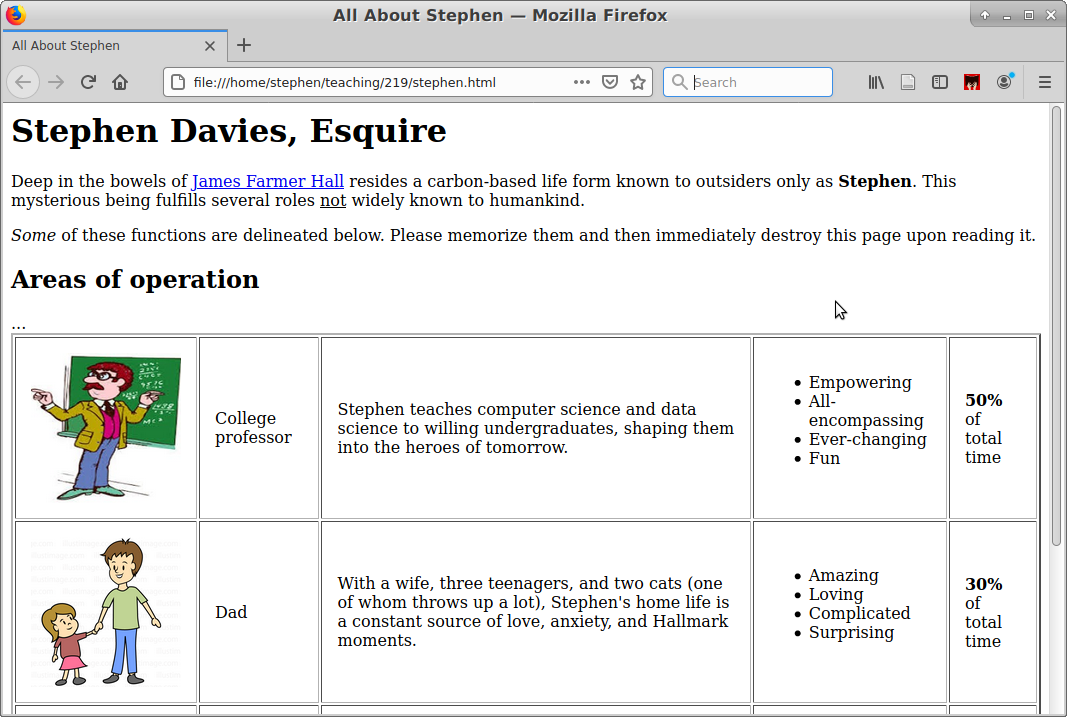
\includegraphics[width=0.9\textwidth]{stephenpage.png}
\end{center}

\section{The easy case: reading from \texttt{<table>}s}

\index{the easy case}
\label{easy2}
\index{screen scraping}

From the point of view of Data Science, we don't care very much about all this
formatting stuff. To us, it's clutter. On the page is some important data we'd
like to analyze, and the goal is to sift through all this HTML and CSS crapola
looking for it and extracting it. This is called by the evocative term
``\textbf{screen scraping}.''

\index{table@\texttt{<table>} (HTML tag)}
\index{table!HTML element}

Now just like with relational databases (recall p.~\pageref{easy1}), there's
both an easy scenario and more challenging ones. The more challenging ones
we'll postpone until the next chapter. The easy one is when the data you want
to scrape \textit{is all inside \textbf{HTML tables}}. 

\index{read\_html@\texttt{read\_html()} (Pandas)}

An HTML table is the contents between an opening \textbf{<table>} tag and its
corresponding \textbf{</table>} tag. Look carefully again at
Figure~\ref{fig:allAboutStephen} on p.~\pageref{fig:allAboutStephen}.
\textit{If} the information we care about scraping is all inside the ``areas of
operation'' table (which begins about half-way down the page; squint until you
see the word \texttt{table}), then we're in the easy case, thank heavens. We
can use Pandas' \texttt{read\_html()} function as follows:

\vspace{-.1in}
\begin{Verbatim}[fontsize=\footnotesize,samepage=true,frame=single,framesep=3mm]
the_tables = pd.read_html("http://theURLtoTheWebpage.html")
\end{Verbatim}
\vspace{-.1in}

\index{URL}
\index{network connection}
\index{directory (folder)}
\index{folder}
\index{extension (filename)}

\index{allAboutStephen@\texttt{allAboutStephen.html}}

\label{downloading}

This function takes just one argument: the \textbf{URL} of the page we want to
scrape. (A URL -- which stands for Uniform Resource Locator -- is another word
for a web page's address, or ``link.'') Sometimes you'll find it more
convenient to first download the page to your local computer, so that you're
not dependent on a network connection (and latency) while you're working on
scraping it. This will normally put a \texttt{.html} (or \texttt{.htm}) file on
your computer, which you can store in the same directory/folder as your
\texttt{.py} file, just as you do with \texttt{.csv} or \texttt{.db} files.
You'll then pass the simple filename (like ``\texttt{allAboutStephen.htm}'') as
the argument to \texttt{read\_html()}.

The return value of this function is \textit{a list of \texttt{DataFrame}s, one
for each \texttt{<table>} on the page.} Read that sentence once again slowly.
In particular, note that the return value is not \textit{a} \texttt{DataFrame},
which many students seem to expect. This is of course because the web page may
well contain \textit{multiple} \texttt{<table>}s, and therefore
\texttt{read\_html()} would need to return multiple \texttt{DataFrame}s.

\index{allAboutStephen@\texttt{allAboutStephen.html}}

Let's try this approach with \texttt{allAboutStephen.html}:

\begin{Verbatim}[fontsize=\small,samepage=true,frame=single,framesep=3mm]
the_tables = pd.read_html(
    "http://stephendavies.org/allAboutStephen.html")
print(len(the_tables))
\end{Verbatim}
\vspace{-.2in}

\begin{Verbatim}[fontsize=\small,samepage=true,frame=leftline,framesep=5mm,framerule=1mm]
1
\end{Verbatim}

There is apparently only one \texttt{<table>} on the page. Let's put it in its
own variable (``\texttt{areas}'' for ``Areas of operation'') and take a look at
it:

\begin{Verbatim}[fontsize=\small,samepage=true,frame=single,framesep=3mm]
areas = the_tables[0]
print(areas)
\end{Verbatim}
\vspace{-.2in}

\begin{Verbatim}[fontsize=\small,samepage=true,frame=leftline,framesep=5mm,framerule=1mm]
    0  ...                  4
0 NaN  ...  50% of total time
1 NaN  ...  30% of total time
2 NaN  ...  10% of total time
3 NaN  ...   5% of total time
4 NaN  ...   5% of total time

[5 rows x 5 columns]
\end{Verbatim}

\index{NaN@\texttt{NaN} (``not a number'')}

This is a bit confusing at first, for several reasons. One is that the columns
don't have names, as we're used to -- just numbers. Another is that most of the
information is omitted from the display (with just ``\texttt{...}''
placeholders). Another is that the first column is entirely \texttt{NaN}
values\footnote{The value \texttt{NaN}, you'll recall, stands for ``not a
number.'' But that phrase is misleading here. Of \textit{course} the value is
not a \textit{number}: why would we expect text on a web page to necessarily be
a number? Really it means ``not a value Python could do anything with.''}.

\pagebreak
The root causes of these conundrums are as follows:

\begin{compactenum}

\item The \texttt{DataFrame} columns don't have names because HTML
\texttt{<table>}s often don't have header cells (delimited with \texttt{<th>}
cells in the first \texttt{<tr>} row), and so \texttt{read\_html()} has no idea
what to name the columns.

\item Most columns are omitted from the \texttt{print()} output because they're
just too long to fit. (Look at p.~\pageref{stephenpage}: that third column has paragraphs in it.)

\item The first column has \texttt{NaN}s because the first column of the
\texttt{<table>} has images in it, not text (again see
p.~\pageref{stephenpage}).

\end{compactenum}

We can \textit{give} the \texttt{DataFrame} meaningful column names with:

\begin{Verbatim}[fontsize=\small,samepage=true,frame=single,framesep=3mm]
areas.columns = ['pic','role','description','adjectives',
    'allocation']
\end{Verbatim}

and we can get rid of the columns we don't care about (the image, and perhaps
the descriptions) with a Pandas operation:

\begin{Verbatim}[fontsize=\small,samepage=true,frame=single,framesep=3mm]
areas = areas[['role','adjectives','allocation']]
\end{Verbatim}

Now we can see better what's going on:

\begin{Verbatim}[fontsize=\small,samepage=true,frame=single,framesep=3mm]
print(areas)
\end{Verbatim}

\vspace{-.2in}

\begin{Verbatim}[fontsize=\scriptsize,samepage=true,frame=leftline,framesep=3mm,framerule=1mm]
             role                        adjectives          allocation
College professor   Empowering  Important  Fun  ...   50% of total time
Dad                            Amazing Fun Impor...   30% of total time
Kids Club Leader    Cute  Exhausting  Character-...   10% of total time
Secret Agent        Thrilling  High-impact  Dang...    5% of total time
Jedi Master         Important  Thrilling  Challe...    5% of total time
\end{Verbatim}

\subsection{Some text cleaning stuff}

At this point, we're out of screen-scraping-land and into ordinary-Python land.
What we do next depends on what we want to analyze. One interesting question I
could imagine asking is: ``how much of Stephen's total time does he spend doing
`fun' things? `important' things? `exhausting' things?

\index{adjectives@\texttt{adjectives}}
\index{ul@\texttt{<ul>} (HTML tag)}
\index{li@\texttt{<li>} (HTML tag)}

To do this, we'll have to deal with that messy \texttt{adjectives} column. I
say it's ``messy'' because all Pandas knew to do was take each bulleted list
-- comprised of a \texttt{<ul>} element (``unordered list'') and nested
\texttt{<li>} elements (``list elements'') -- and concatenate all the contents
into a single string.

My strategy to dealing with it is to split these up, putting each role's
adjective in its own row of a new table that looks like this:

\begin{Verbatim}[fontsize=\small,samepage=true,frame=leftline,framesep=5mm,framerule=1mm]
                   role           adjective
      College professor          Empowering
      College professor           Important
                    Dad             Amazing
       Kids Club Leader           Important
                   . . . etc . . .
\end{Verbatim}

\index{object@``\texttt{object}'' (a.k.a. \texttt{str}) \texttt{dtype}}
\index{append@\texttt{append()} (NumPy)}
\index{array@\texttt{array()} (NumPy)}

We can do this with a loop. Since we don't know at the beginning how many rows
this table will have, we'll use a slightly different technique than we did on
p.~\pageref{objectDtype}. We'll just create two \textit{zero}-length NumPy
arrays, and repeatedly \texttt{append()} to them for each new adjective we
encounter:

\begin{Verbatim}[fontsize=\small,samepage=true,frame=single,framesep=3mm]
roles = np.array([], dtype=object)
adjs = np.array([], dtype=object)

for row in areas.itertuples():
    for adjective in row.adjectives.split():
        roles = np.append(roles, row.role)
        adjs = np.append(adjs, adjective)
\end{Verbatim}

\pagebreak
Two other notable things about this code:

\begin{compactitem}

\index{nested!loops}

\item It's a \textit{nested} \texttt{for} loop. This is because (1) we have to
go through all the rows of our \texttt{areas} \texttt{DataFrame}, and (2) for
each of those rows, there will be \textit{multiple} adjectives.

\index{split@\texttt{.split()}}
\index{delimiter}
\index{list}

\item We use the very handy \texttt{.split()} method here. When you call
\texttt{.split()} on a string, you get back all its individual words in a
list. You can also pass an argument to \texttt{.split()} giving the
string \textbf{delimiter} that you want it to divide the string on. So calling
\texttt{"needles/yarn/scissors".split("/")} would return the list
\texttt{["needles", "yarn", "scissors"]}, and calling
\texttt{"Stephen".split("e")} would return the list \texttt{["St", "ph",
"n"]}.

\end{compactitem}

\index{stitching arrays together}

Now all we have to do is stitch together our arrays into a \texttt{DataFrame},
just like we did on p.~\pageref{stitching}:

\index{adjectives\_df@\texttt{adjectives\_df}}

\begin{Verbatim}[fontsize=\footnotesize,samepage=true,frame=single,framesep=3mm]
adjectives_df = pd.DataFrame({'role':roles, 'adjective':adjs})
\end{Verbatim}
\vspace{-.2in}

and voil\`{a}! The resulting \texttt{adjectives\_df} is in
Figure~\ref{adjectives_df}.

\begin{figure}[ht]
\centering
\begin{Verbatim}[fontsize=\footnotesize,samepage=true,frame=leftline,framesep=5mm,framerule=1mm]
                             role           adjective
            0   College professor          Empowering
            1   College professor           Important
            2   College professor                 Fun
            3   College professor                Cool
            4   College professor    All-encompassing
            5   College professor       Ever-changing
            6                 Dad             Amazing
            7                 Dad                 Fun
            8                 Dad           Important
            9                 Dad         Challenging
            10   Kids Club Leader                Cute
            11   Kids Club Leader          Exhausting
            12   Kids Club Leader  Character-building
            13   Kids Club Leader           Important
            14       Secret Agent           Thrilling
            15       Secret Agent         High-impact
            16       Secret Agent           Dangerous
            17       Secret Agent                Cool
            18       Secret Agent              Daring
            19        Jedi Master           Important
            20        Jedi Master           Thrilling
            21        Jedi Master         Challenging
            22        Jedi Master              Daring
            23        Jedi Master                Cool
            24        Jedi Master                 Lit
\end{Verbatim}
\caption{The \texttt{adjectives\_df} \texttt{DataFrame} we constructed with our
nested \texttt{for} loop.}
\label{adjectives_df}
\end{figure}

And now that we've done that, we can get rid of the old, awkward,
separated-by-spaces column:

\begin{Verbatim}[fontsize=\footnotesize,samepage=true,frame=single,framesep=3mm]
areas = areas[['role','allocation']]
\end{Verbatim}

Okay. The other thing we need to do is change those ridiculous human-readable
strings like ``\texttt{30\% of total time}'' to integers like \texttt{30}.
We'll use the \texttt{.split()} method again, this time passing a delimiter:

\index{split@\texttt{.split()}}
\index{delimiter}

\begin{Verbatim}[fontsize=\footnotesize,samepage=true,frame=single,framesep=3mm]
percentages = np.array([], dtype=int)

for row in areas.itertuples():
    percentages = np.append(percentages,
        int(row.allocation.split("%")[0]))

areas.allocation = percentages
\end{Verbatim}

What does ``\texttt{int(row.allocation.split("\%")[0])}'' mean? Let's break it
down. For each row, we first get the allocation column's value (which is a
string), then split it on the ``\texttt{\%}'' sign. This will give us a list of
two values in each case, the first of which has digits like ``\texttt{30}'' and
the second of which has the rest of the text (``\texttt{of total time}'').
Putting \texttt{[0]} after it gets the first element of this list. Then, by
wrapping the result in ``\texttt{int(...)}'', we convert it from a string of
digits to an actual number, which we can do something with.

\smallskip
The last step in that code was to reassign the \texttt{DataFrame}'s
\texttt{allocation} column to be our new percentages. The result is now:

\begin{Verbatim}[fontsize=\small,samepage=true,frame=single,framesep=3mm]
print(areas)
\end{Verbatim}

\begin{Verbatim}[fontsize=\small,samepage=true,frame=leftline,framesep=5mm,framerule=1mm]
                                role  allocation
                0  College professor          50
                1                Dad          30
                2   Kids Club Leader          10
                3       Secret Agent           5
                4        Jedi Master           5
                               .  .  .
\end{Verbatim}

where the right-most column actually has numbers.

\subsection{The analysis}

\index{adjectives\_df@\texttt{adjectives\_df}}
\index{merge}

Finally (whew!) we're in a position to perform our analysis of Stephen's time.
We have two \texttt{DataFrames} -- \texttt{areas} and \texttt{adjectives\_df}
-- both of which are needed to answer our key question. So it makes sense to
merge them. It now sucks to have the role be the index of the \texttt{areas}
\texttt{DataFrame}, so let's make it a regular column again and then do the
merge:

\label{roles_df}

\begin{Verbatim}[fontsize=\small,samepage=true,frame=single,framesep=3mm]
df = pd.merge(areas, adjectives_df)
print(df)
\end{Verbatim}
\vspace{-.2in}

\begin{Verbatim}[fontsize=\footnotesize,samepage=true,frame=leftline,framesep=5mm,framerule=1mm]
                         role  allocation           adjective
        0   College professor          50          Empowering
        1   College professor          50           Important
        2   College professor          50                 Fun
        3   College professor          50                Cool
        4   College professor          50    All-encompassing
        5   College professor          50       Ever-changing
        6                 Dad          30             Amazing
        7                 Dad          30                 Fun
                                   .  .  .
\end{Verbatim}

And at last, after all this data cleaning, we can get the goods. The
\textit{number} of different roles Stephen plays that have various adjectives
is as follows:

\begin{Verbatim}[fontsize=\footnotesize,samepage=true,frame=single,framesep=3mm]
print(df.adjective.value_counts())
\end{Verbatim}
\vspace{-.2in}

\begin{Verbatim}[fontsize=\scriptsize,samepage=true,frame=leftline,framesep=5mm,framerule=1mm]
            Important             4
            Cool                  3
            Fun                   2
            Thrilling             2
            Challenging           2
            Daring                2
            High-impact           1
            Amazing               1
            Ever-changing         1
            Cute                  1
            Lit                   1
            Exhausting            1
            Empowering            1
            All-encompassing      1
            Character-building    1
            Dangerous             1
\end{Verbatim}

And the \textit{percentage} of time he spends with these adjectives is:

\begin{Verbatim}[fontsize=\footnotesize,samepage=true,frame=single,framesep=3mm]
perc_of_time = df.groupby('adjective').allocation.sum()
print(perc_of_time.sort_values(ascending=False))
perc_of_time.plot(kind='bar')
\end{Verbatim}
\vspace{-.2in}

\begin{Verbatim}[fontsize=\scriptsize,samepage=true,frame=leftline,framesep=5mm,framerule=1mm]
            Important             95
            Fun                   80
            Cool                  60
            Ever-changing         50
            Empowering            50
            All-encompassing      50
            Challenging           35
            Amazing               30
            Thrilling             10
            Exhausting            10
            Daring                10
            Cute                  10
            Character-building    10
            Lit                    5
            High-impact            5
            Dangerous              5
\end{Verbatim}

which is represented in Figure~\ref{fig:adjectives}.

\begin{figure}[ht]
\centering
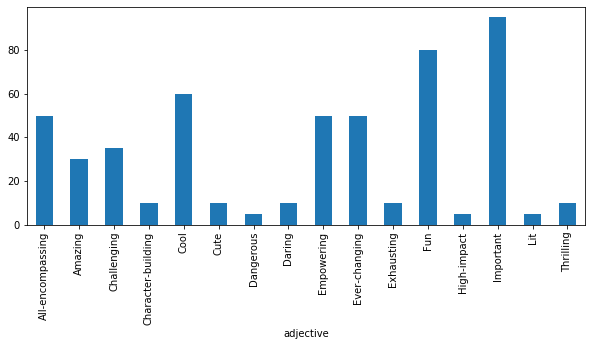
\includegraphics[width=0.7\textwidth]{adjectives.png}
\caption{Good news: Stephen spends a lot of time doing important stuff!}
\label{fig:adjectives}
\end{figure}

I know that might seem like a lot of work for ``the easy case.'' But the wild
wild world has lots of messiness, and if you want the data shown on a web page
you have to put in some elbow grease to bend it to your will. The good news is
that as far as scraping the actual \textit{page}, all we needed was one
command: \texttt{pd.read\_html()}. If the data you want from a page isn't in
\texttt{<table>}s, though, you're in for the tougher case in
Chapter~\ref{ch:screenScraping2}. Stay tuned!

